\section{Modelado y simulación de un sistema de calentamiento solar}
\begin{enumerate}
   \item Modele matemáticamente el sistema de calentamiento, tomando como variable
         de salida la temperatura $\theta(t)$\label{item_2_1}
   \item Halle el flujo de calor por radiación necesario para obtener en estado
         estacionario una temperatura de salida $\theta_{ref}=60^{\circ}C$\label{item_2_2}
   \item Obtenga el tiempo necesario para alcanzar dicha temperatura, si el
         fluido a calentar se encuentra a $\theta_{0}=15^{\circ}C$\label{item_2_3}
   \item En época invernal la radiación solar se reduce notablemente y es
         insuficiente para alcanzar la temperatura deseada. Considere una situación en donde la
         radiación es del $40\%$ de la obtenida en el item anterior, y la temperatura inicial del
         fluído es de $15^{\circ}C$. Cual es la temperatura de estado estacionario en estas
         condiciones?\label{item_2_4}
   \item Diseñe un circuito que complemente el colector solar para lograr la temperatura deseada
         de $60^{\circ}C$. Cuando el sistema de calentamiento se encuentra funcionando en lazo
         abierto, cualquier pequeña perturbacion en las condiciones teóricas de operación produce
         una desviación no deseada en la temperatura estacionaria de salida. Por este motivo,
         se ha introducido un controlador PI para garantizar el seguimiento de la consigna de
         temperatura en estado estacionario. De esta manera, una vez cerrado el lazo, la potencia
         calorífica que se suministra al circuito complementario es calculada directamente por el
         algoritmo de control y la nueva variable de entrada al sistema es entonces la temperatura
         de referencia $\theta_{ref}$\label{item_2_5}
   \item Modele matemáticamente el sistema a lazo cerrado, tomando como variable de salida la
         temperatura $\theta(t)$ y como variable de entrada su valor de referencia $\theta_{ref}$\label{item_2_6}
   \item Simule la evolución dinámica de la temperatura del sistema desde un instante inicial
         $\theta_{0}$ hasta un valor de referencia $\theta_{ref}$, operando en lazo abierto y
         en lazo cerrado, para tres valores distintos de ambas temperaturas.\label{item_2_7}
   \item Estudie el comportamiento del sistema a lazo abierto y a lazo cerrado frente a
         perturbaciones de tipo escalón y rampa en la variable de entrada.¿Qué conclusión extrae
         de la eficiencia del controlador PI en ambos casos?¿Que sucedería si se utiliza sólo
         acción proporcional?\label{item_2_8}
\end{enumerate}

\begin{figure}[H]
   \centering
   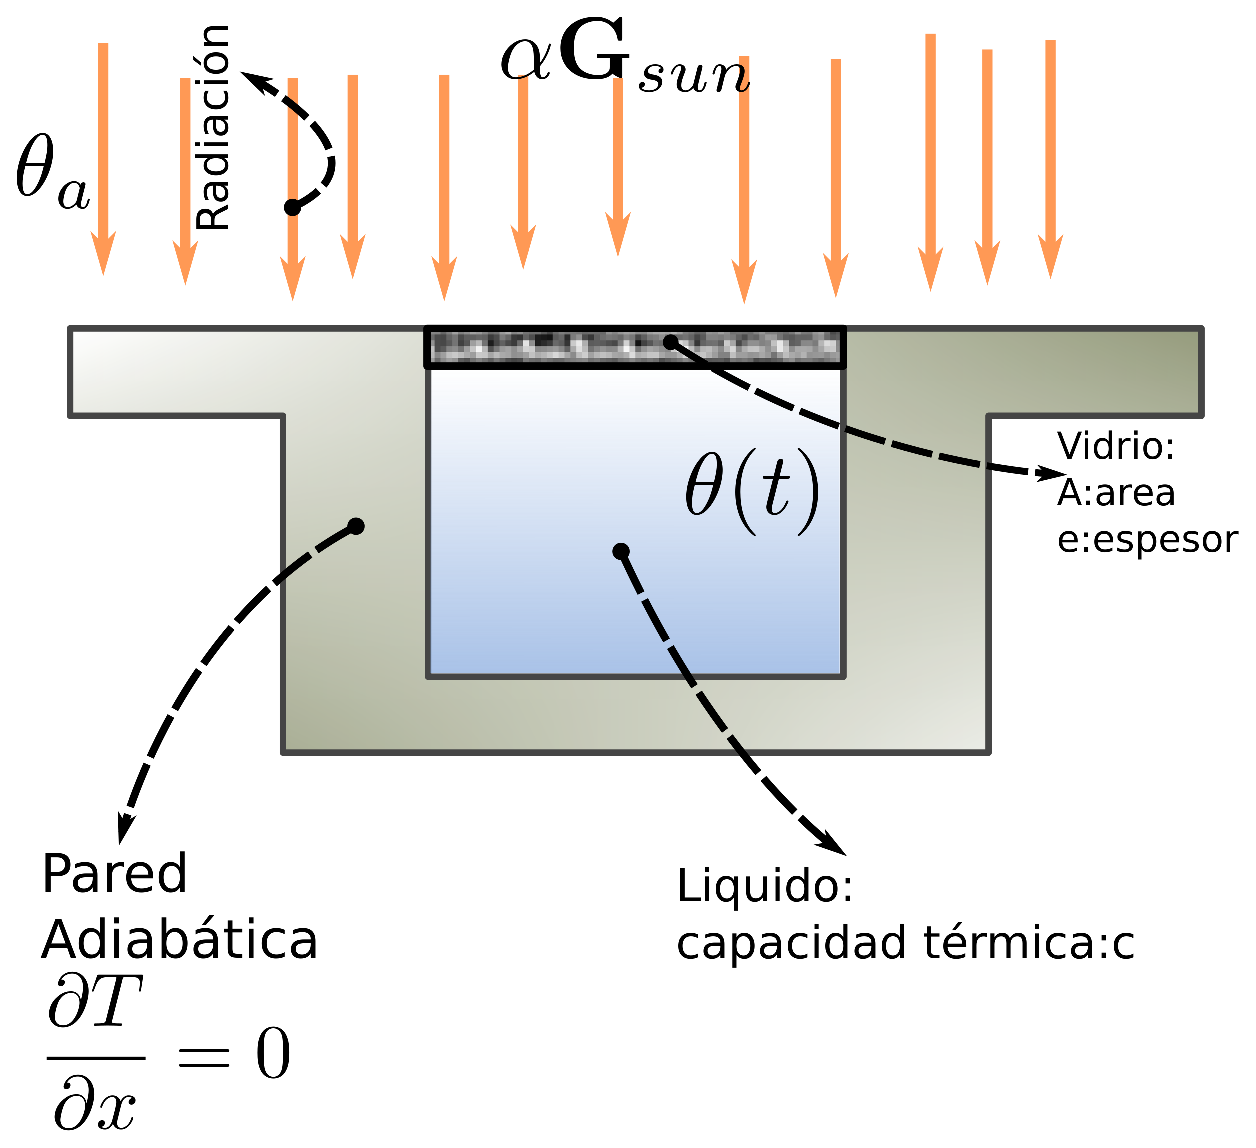
\includegraphics[width=0.37\textwidth]{Images/colector_esquema.eps}
   \caption{Esquema del colector solar}\label{fig:colector_esquema}
\end{figure}
%------------------------------------------------------------------------------
%                      resolucion problema 2
%------------------------------------------------------------------------------
\subsection{Resolución}
\subsubsection{\ref{item_2_1}-Modelado del problema}
Para modelar matemáticamente el sistema de calentamiento, planteamos un balance de energía alrededor
del agua del colector (cuyo Volumen de Control se muestra en la fig[\ref{fig:colector_esquema}]),
eligiendo una base de tiempos diferencial:
\begin{equation}
   \dot{E}_{e} - \dot{E}_{s}=\dot{E}_{a}\label{eq:balance}
\end{equation}
Donde:
\begin{equation}
   \dot{E}_{e} = G\,A\label{eq:balance_entrada}
\end{equation}
\begin{equation}
   \dot{E}_{s} = \dfrac{\theta(t) - \theta_{a}}{R}\label{eq:balance_salida}
\end{equation}
\begin{equation}
   \dot{E}_{a} = c_{e}\,V\,\dfrac{d\theta(t)}{dt}\label{eq:balance_acumulacion}
\end{equation}
Entonces reemplazando [\ref{eq:balance_entrada}], [\ref{eq:balance_salida}] y
[\ref{eq:balance_acumulacion}] en [\ref{eq:balance}] obtenemos la siguiente ecuación diferencial:

\begin{equation}
   G\,A - \dfrac{\theta(t) - \theta_{a}}{R} = c_{e}\,V\,\dfrac{d\theta(t)}{dt}\label{eq:balance_completo}
\end{equation}
Que podemos expresar:
\begin{equation}
   \dfrac{d\theta(t)}{dt} = \dfrac{G\,A}{c_{e}\,V} + \dfrac{\theta_{a}}{R\,c_{e}\,V} - \dfrac{\theta(t)}{R\,c_{e}\,V}
   \label{eq:modelo_problema2}
\end{equation}
\subsubsection{\ref{item_2_2}-Flujo de calor por radiación}
Para obtener en estado estacionario una temperatura de salida $\theta_{ref}=60\degree C$. De la ecuación que
modela el problema[\ref{eq:modelo_problema2}], la condición que se debe cumplir en estado estacionario
es $\dfrac{d\theta(t)}{dt} = 0$, donde en este caso se quiere que $\theta(t)=\theta_{ref}$ entonces
reemplazando nos queda:
\begin{align}
   0 &= \dfrac{G_{nec}\,A}{c_{e}\,V} + \dfrac{\theta_{a}}{R\,c_{e}\,V} - \dfrac{\theta(t)}{R\,c_{e}\,V}\\
   0 &= G_{nec} \, A + \dfrac{\theta_{a}-\theta_{ref}}{R}\\
   G_{nec} &= \dfrac{\theta_{ref}-\theta_{a}}{R\,A}\label{eq:flujo_necesario}
\end{align}
Reemplazando los valores dados nos queda:
\begin{equation}
   G_{nec} = 836800 \,[W/m^{2}]
\end{equation}
Con este valor calculado se simula el sistema cuya grafica es la siguiente:

\begin{figure}[H]
   \centering
   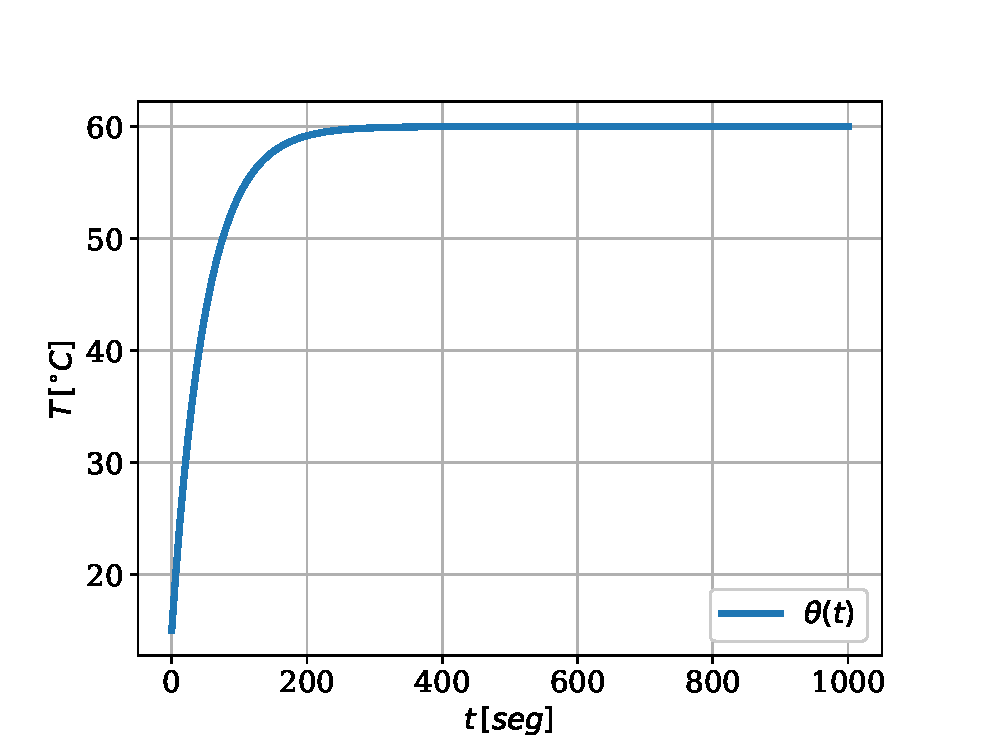
\includegraphics[width=0.67\textwidth]{Images/temperatura_colector.eps}
   \caption{Temperatura colector solar}\label{fig:colector_temperatura}
\end{figure}


\subsubsection{\ref{item_2_3}-tiempo para alcanzar la temperatura $\theta_{ref}$}
Si bien del grafico se puede ver que alcanza el valor, no esta claro en que momento exacto llega a ese valor,
por ello se realizo una simulación numérica del mismo para verificar exactamente cuando
alcanza el valor. El resultado que se obtuvo es (con una tolerancia de $10e-12$): $t_a =571.312[seg]$
(\verb|Programas/problema2_tiempo_60.jl|)

\subsubsection{\ref{item_2_4}-Perfil de temperatura en epoca invernal}
En epocas invernales tenemos las siguientes variantes:

\begin{itemize}
   \item $G_{inv}=0.4\,G_{nec}$
   \item $\theta_{0} = 8 \degree C$
\end{itemize}
Simulando el sistema con estos valores nos genera el siguiente perfil de temperatura:

\begin{figure}[H]
   \centering
   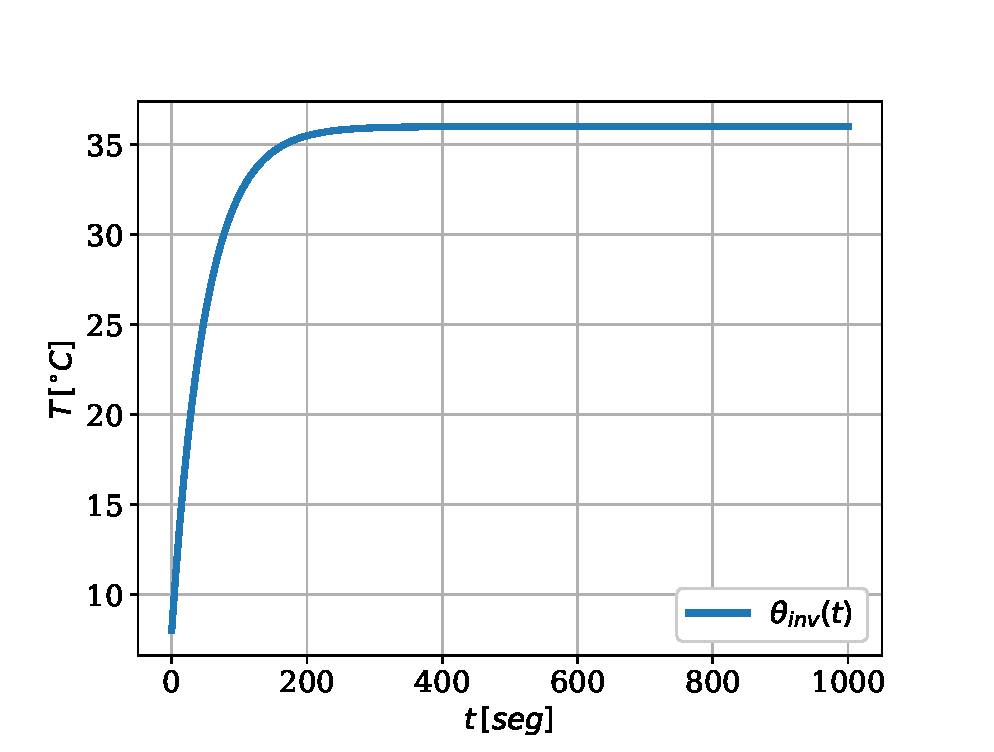
\includegraphics[width=0.67\textwidth]{Images/temperatura_colector_invierno.eps}
   \caption{temperatura colector solar en invierno}\label{fig:colector_temperatura_invierno}
\end{figure}

cuya solución numérica nos arroja el valor final de temperatura: $\theta_{inv} = 35.999 \degree C$

(\verb|Programas/problema2_simulacion_calentamiento_invierno.jl|)

La potencia necesaria adicional que necesitamos para llegar a la temperatura deseada $\theta_{ref}$, la podemos calcular
planteando condiciones de estado estable ($\dfrac{d\theta}{dt}=0$) en el balance de energía osea:
\begin{align}
   q_{nec}+\,A\,G_{inv}&=\dfrac{\theta_{ref}-\theta_{a}}{R}\\
   q_{nec}&=\frac{\theta_{ref}-\theta_{a}}{R}-\,A\,G_{inv}\\
   q_{nec}&=1.00416e6\,[W]
\end{align}
Verificamos que con ese valor de potencia colorica agregada obtemos el valor final deseado para el perfil de temperatura

\begin{figure}[H]
   \centering
   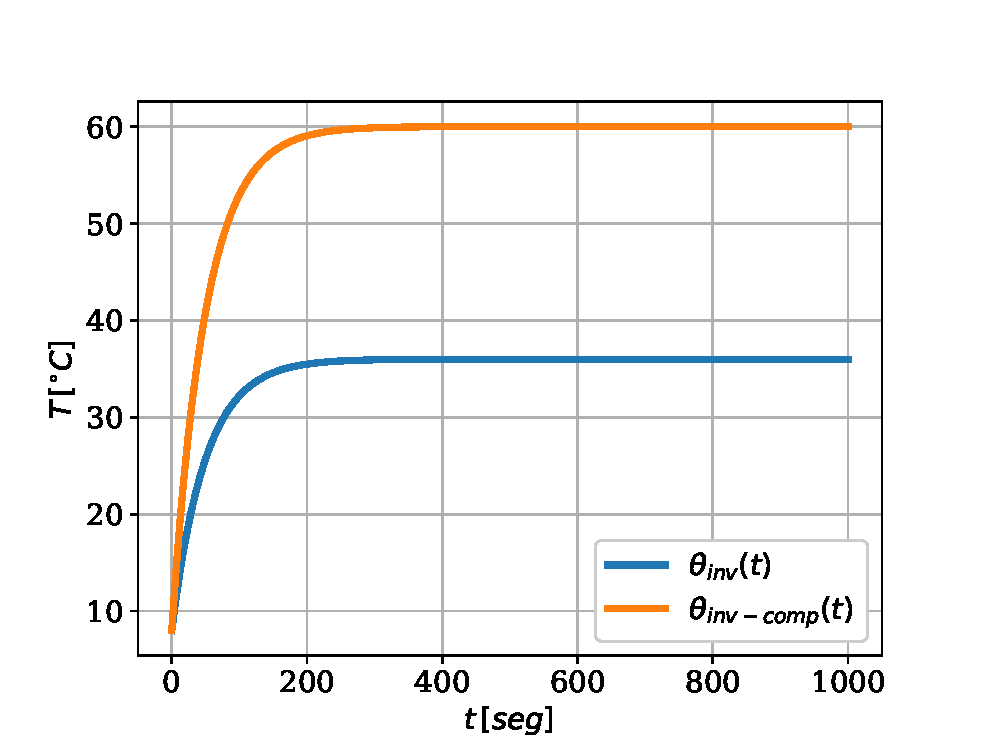
\includegraphics[width=0.67\textwidth]{Images/colector_esquema_invierno_comp.eps}
   \caption{temperatura colector solar en invierno y temperatura compensada}\label{fig:colector_temperatura_invierno_comp}
\end{figure}

%------------------------------------------------------------------------------
%                      2_5
%------------------------------------------------------------------------------
\subsubsection{\ref{item_2_5}-Diseño de Circuito complementario}
De los resultados anteriores se pudo observar que no es posible alcanzar los niveles de temperatura
deseada en invierno, por ello para cumplir con ese requerimiento debemos agregar una fuente de generación de
calor externa. Una de las posibles soluciones es agregar un sistema de calentamiento simple, que
consiste en el calentamiento de una resistencia electrica dentro del colector de agua. La fuente
de corriente podría provenir de una placa fotovoltaica instalada al lado del colector solar
Gráficamente:

\begin{figure}[H]
   \centering
   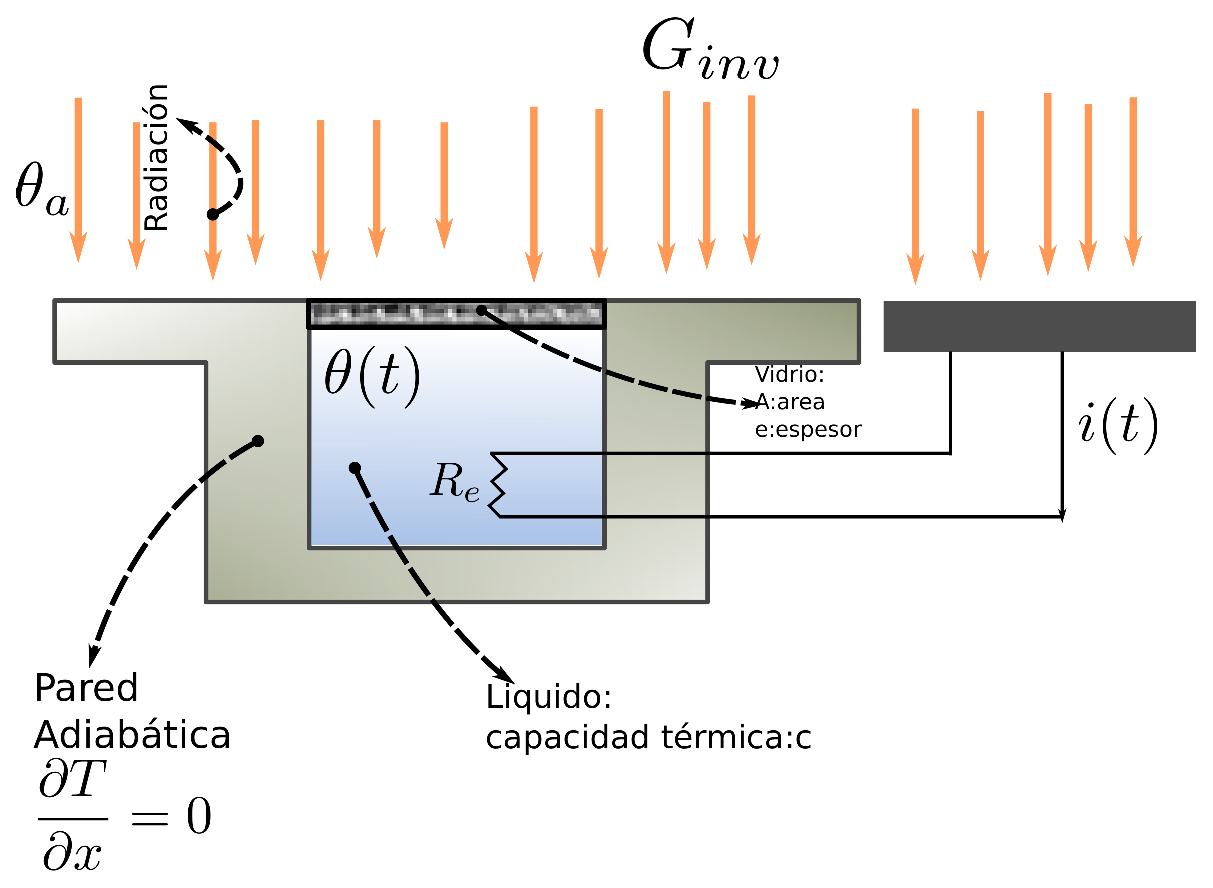
\includegraphics[width=0.47\textwidth]{Images/colector_esquema_invierno.eps}
   \caption{Colector solar alternativo para el invierno}\label{fig:colector_esquema_invierno}
\end{figure}
La fuente de calor externa entonces se puede expresar en función del tiempo:
\begin{equation}
   q(t) = R_{e}\,\left(i(t)\right)^{2}
\end{equation}
Ahora el balance de energía se modifica ya que hemos agregado una fuente de calor, por ello nos queda:

\begin{equation}
   q(t)+ A\,G_{inv}-\dfrac{\theta(t)-\theta_{a}}{R}=c_e\,V\,\dfrac{d\theta(t)}{dt}\label{eq:balance_close_loop}
\end{equation}

\subsubsection{\ref{item_2_6}-Modelo a lazo cerrado}
A lazo cerrado la señal de control que nos permite regular la temperatura del colector solar:
\begin{equation}
   q(e(t))=K_p\,e(t)+K_i\,\int_0^{t}\,e(\alpha)\,d\alpha
\end{equation}
Donde:
\begin{equation}
   e(t) = (\theta_{ref}(t)-\theta(t))
\end{equation}
Entonces reemplazando en [\ref{eq:balance_close_loop}] nos queda:
\begin{equation}
   K_p\,e(t)+K_i\,\int_0^{t}\,e(\alpha)\,d\alpha + A\,G_{inv}-\dfrac{\theta(t)-\theta_{a}}{R}=c_e\,V\,\dfrac{d\theta(t)}{dt}
   \label{eq:close_loop}
\end{equation}
%------------------------------------------------------------------------------
%                      fin problema 2
%------------------------------------------------------------------------------

